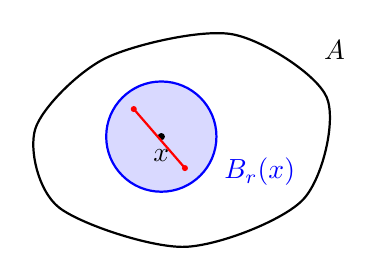
\begin{tikzpicture}[scale=1]
\draw[thick] plot[smooth cycle] coordinates {(0,0) (1.6,-0.5) (3.1,0.1) (3.4,1.4) (2.2,2.2) (0.6,1.9) (-0.3,1)};
\node at (3.5,2.0) {$A$};
\fill[blue, fill opacity=0.15] (1.3,0.9) circle (0.7);
\draw[blue, thick] (1.3,0.9) circle (0.7);
\fill (1.3,0.9) circle (1.3pt) node[below=1pt] {$x$};
\node[blue] at (2.55,0.45) {$B_r(x)$};
\fill[red] (0.95,1.25) circle (1.1pt);
\fill[red] (1.6,0.5) circle (1.1pt);
\draw[red, thick] (0.95,1.25) -- (1.6,0.5);
\end{tikzpicture}
